\documentclass[11pt]{article}
\usepackage[a4paper, total={6in, 8in}]{geometry}
\usepackage{amsmath}
\usepackage{amsthm}
\usepackage{graphicx}
\usepackage{amsfonts}
\usepackage{xcolor}
\begin{document}

\newtheorem{theorem}{Theorem}
\numberwithin{theorem}{section}
\theoremstyle{definition}
\newtheorem{definition}{Definition}
\newtheorem{proposition}{Proposition}
\newtheorem{example}{Example}
\newtheorem{lemma}{Lemma}
\newtheorem{corollary}{Corollary}
\numberwithin{definition}{section}
\numberwithin{proposition}{section}
\numberwithin{example}{section}
\numberwithin{lemma}{section}
\numberwithin{corollary}{section}
\newcommand{\uw}{\mathcal{U}(W,X)}
\newcommand{\W}{$(W,S)$}
\newcommand{\ix}{\textit}
\newcommand{\tr}{\textcolor{red}}
\newcommand{\sg}{$\Sigma$}


\title{Shadows in Coxeter Complexes}
\maketitle
\tableofcontents 



\textcolor{red}{Red notes for Megan}

\textcolor{blue}{Blue notes for Yusra}

Figures are not my own. \tr{Should I produce my own? Which software would you recommend?}

\section{Coxeter complexes}
\begin{definition}
    Let $(W,S)$ be a Coxeter system. Let $S'\subset S$. We define the \textit{standard parabolic subgroup} $W_{s'}$ of $W$ to be the subgroup generated by the subset $S'$. Then $(W_{s'},S')$ is also a Coxeter group. 
\end{definition}

We can now define an abstract simplicial complex $\Sigma$ by taking all the left cosets $xW_{S'}$ of all the standard parabolic subgroups, and defining a partial order on this set by reverse inclusion. 


The vertex set of this simplicial complex corresponds to cosets of the maximal parabolic subgroups. These maximal parabolic subgroups are formed by taking a subset of $S$ with one element removed. So these maximal parabolic subgroups are in bijection with the elements of $S$. 


\begin{definition}
    The maximal simplicies in the simplicial complex are called \textit{alcoves}, and the codimension-one faces are called \textit{panels}.  
\end{definition}

We note that there is a correspondence between between panels and vertices. This is because a vertex corresponds to an element of the form $xW_{S\backslash \{s\}}$, whilst a panel corresponds to an element of the form $xW_{S\backslash \{s\}}$. 

\begin{definition}
    If a panel $p$ corresonds to the element $xW_{S\backslash \{s\}}$, we say that $p$ has \ix{type} $s$, and write $\tau(p)=s$. 
\end{definition}

Then we can consider $W$ acting on this simplicial complex.
We want to consider the set of elements of $W$ which exactly fix a hyperplane in the simplicial complex. This subset is
\[R:=\bigcup_{x\in W}xSx^{-1},\]
and the elements of this set are called \ix{reflections}. Given an element $r\in R$, we denoted the hyperplane it fixes by $H_r$. Then the hyperplane $H_r$ \ix{separates} two alcoves if they are contained in different half-spaces defined by $H_r$. 

Now let us consider a Euclidean Coxeter system of type $\tilde{X}$. This group can be split into a semi-direct product of a spherical Weyl group $W_0$ and a translation group $T$ which acts on $\Sigma$.
\begin{definition}
    A vertex of $\Sigma$ whose stabiliser in $W$ is isomorphic to $W_0$ is called a \ix{special vertex}.
\end{definition}

Now when we have an irreducible Euclidean Coxeter system, $\Sigma$ can be geometrically realised as a tiling of the Euclidean $n$-space, where $n=|S|-1$. Now here, the group $T$ is isomorphic to $\mathbb{Z}^n$. This corresponds to the coroot lattice. 

Let us consider this geometric realisation of $\Sigma$, which we also call $\Sigma$. Then we fix a special vertex 0, which we call the \ix{origin} of $\Sigma$. We want to consider the set $\mathcal{H}_v$ of all hyperplanes through a special vertex $v$ which is in the orbit of 0 under $T$. 

\begin{definition}
    The \ix{Weyl chambers} are the closures of the connected components of \[\Sigma\backslash \cup_{H\in\mathcal{H}}H.\]
\end{definition}

\tr{Is it not a little confusing to call the special alcoves 'Weyl chambers', instead of 'Weyl alcoves'?}

Now the set of equivalence classes of parallel rays in $\Sigma$ form what we call the \ix{boundary sphere}, denoted by $\partial\Sigma$. This sphere inherits a tiling from the oirginal tiling of the Euclidean plane. To do this, we take, as the hyperplanes, the parallel classes of hyperplanes in $\Sigma$. 
Now the maximal simplicies of the boundary sphere are just the parallel classes of Weyl chambers in \sg. We then refer to these maximal simplicies of the boundary as \ix{chambers}.


We can identify the alcoves of $\Sigma$ with elements of $W$, and similarly identify chambers of $\partial\Sigma$ with elements of $W_0$, such that these idenfications are compatible. For instance, we identify the identity element to the chamber of $\partial\Sigma$ which has representative the fundamental Weyl chamber. 


\section{Orientations}

For this section, let $(W,S)$ be any Coxeter system, and $\Sigma$ be its associated Coxeter complex.

\begin{definition}
    An \ix{orientation} $\phi$ of $\Sigma$ is a map from the set of pairs $(p,c)$, where $p$ is a panel and $c$ is an alcove containing $p$, to the set $\{+1,-1\}$. If $\phi (p,c)=+1$, then we say that $c$ is on the $\phi$-\ix{positive side}, otherwise we say that $c$ is on the $\phi$-\ix{negative side}. 
\end{definition}


\begin{example}
    The trivial positive orientation is the map which sends all pairs to $+1$. Similarly, the trivial negative orientation is the map which sends all pairs to $-1$. 
\end{example}

Often, we do not want to have orientations which locally behave like trivial orientations. Hence, we define the following concept:

\begin{definition}
    Given an orientation $\phi$ of \sg, we have
    \begin{enumerate}
        \item $\phi$ is \ix{locally non-negative} if, for each panel, there is at least one alcove which is on the $\phi$-positive side.
        \item $\phi$ is \ix{locally non-trivial} if, for every panel, there is exactly one alcove which is on the $\phi$-positive side.
    \end{enumerate}
\end{definition}


There is a natural action of $W$ on the set of all possible orientations of \sg, induced by the action of $W$ on on the alcoves and panels. It is defined as 
\[(x\cdot\phi)(p,c):=(x^{-1}p,x^{-1}c).\]

\begin{definition}
    Given an orientation $\phi$ of \sg, we say that $\phi$ is \ix{wall consistent} if, given any wall $H$, for all pairs $c,d$ of alcoves which lie in the same halfspace of $H$, with panels $p$ and $q$ respectively, we have that $\phi(p,c)=\phi(q,d)$. If our orientation is wall consistent, we can then define the \ix{positive side} $H^{\epsilon}$ of $H$ as the half-space such that all alcoves $c$ in $H^{\epsilon}$ have $\phi(p,c)=+1$ for all panels of $c$. Then the \ix{negative side} is defined similarly.
\end{definition}

We want to look at several natural ways to orient a Coxeter complex. First, we will look at an orientation which is derived from either a choice of alcove, or a choice of panel. This orientation works for any Coxeter group.

\begin{definition}
    Choose a fixed alcove $c$ in \sg. Now given any alcove $d$, and panel $p$, we define their orientation as $\phi(p,d)=+1$ if and only if $c$ and $d$ lie in the same side of the wall which is spanned by $p$. We call this orientation the \ix{alcove orientation towards c}.
\end{definition}

\tr{Are walls and hyperplanes the same thing? Or is there a difference to how we think of them?}

\begin{definition}
    Choose a fixed simplex $b$ in \sg. Now given any alcove $c$, and panel $p$ in $c$, we define their orientation as $\phi(q,c)=+1$ if and only if either $c$ and $b$ lie in the same side of the wall $H$ containing $p$, or if $b$ lies inside $H$. We call this orientation the \ix{simplex orientation towards b}.
\end{definition}
\begin{example}
    Here we see two simplex orientations of an $A_2$ Coxeter complex. In this complex, the alcoves are edges, and the panels are vertices.
\end{example}
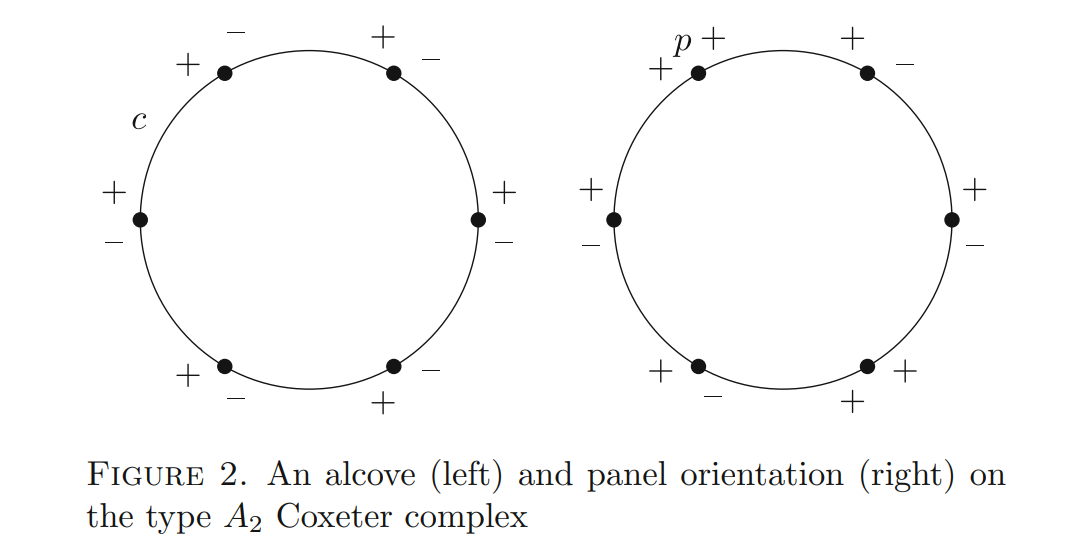
\includegraphics[scale=0.6]{Screenshot 2023-02-03 102201.png}\\

\begin{lemma}
    Consider a Coxeter group $(W,S)$ with Coxeter complex \sg. We have the following:
    \begin{enumerate}
        \item If $\phi$ is a simplex orientation of \sg, then $\phi$ is wall consistent and locally non-negative.
        \item If $\phi$ is an alcove orientation of \sg, then $\phi$ is wall consistent and locally non-trivial.
    \end{enumerate}
\end{lemma}

\subsection{The affine case}

Now we want to consider when our Coxeter complex $\Sigma$ is affine. To define an orientation on \sg, we choose a chamber at infinity.

If $\phi$ is a wall consistent orientation, then, given two chambers $c,d$ which share a common panel $p$, $c$ and $d$ are given the same orientation if they lie in the same half-space of the hyperplane spanned by $p$. This amounts to picking a positive side of the hyperplane.

However, we did not have to pick these positive sides in any consistent way. 

\begin{definition}
    Let $\phi$ be a wall consistent orientation of an affine Coxeter complex. We say that $\phi$ is \ix{periodic} if, given two parallel hyperplanes $H_1,H_2$ and corresponding half-spaces $H_1^{\epsilon},H_2^{\epsilon}$, if $H_1^{\epsilon}\subset H_2^{\epsilon}$, then $H_1^{\epsilon}$ is positive if and only if $H_2^{\epsilon}$ is positive. 
\end{definition}

\begin{example}
    If $\phi$ is a trivial orientation on an affine Coxeter complex, then $\phi$ is periodic. 
\end{example}

\begin{example}
    Simplex orientations are not periodic, as, for every set of parallel hyperplanes, we can find pairs of representatives which have the simplex on different sides.
\end{example}

If $\phi$ is a periodic orientation, then we have a natural orientation induced on the boundary, and vice versa. 

\begin{lemma}
    Given a periodic orientation $\phi$ on an affine Coxeter complex \sg, there is an induced wall-consistent orientation $\partial\phi$ on the boundary complex $\partial\Sigma$. Now if $\phi$ is locally non-negative or non-trivial, so is $\partial\phi$. 
\end{lemma}

\begin{lemma}
    Given a wall-consistent orientation $\phi$ of the boundary complex $\partial\Sigma$, there exists a unique periodic orientation $\tilde{\phi}$ of \sg, which induces the orientation $\phi$. 
\end{lemma}

\begin{definition}
    Let $\sigma$ be a chamber of the boundary $\Delta$ of a Coxeter complex \sg. Then we form an orientation $\phi_{\sigma}$ on the boundary $\Delta$. The \ix{Weyl chamber orientation} on $\Sigma$ is the induced orientation by $\phi_{\sigma}$. 
\end{definition}

\section{Folded galleries}

\subsection{Definitions}
\begin{definition}
    Given a Coxeter complex \sg, a \ix{combinatorial gallery} is a sequence
    \[\gamma = (c_0,p_1,c_1,p_2,...,p_n,c_n),\]
    where the $c_i$ are alcoves and the $p_i$ are panels of \sg, such that $p_i$ is contained in $c_i$ and $c_{i-1}$ for all $i-1,...,n$. The length of a combinatorial gallery $\gamma$ is $n+1$ - this counts how many alcoves there are in the sequence. Then $\gamma$ is \ix{minimal} if there does not exist a shorter gallery starting at $c_0$ and ending at $c_n$. 
\end{definition}

So a gallery is a path between $c_0$ and $c_n$ through alcoves, such that adjacent alcoves in the path share a commmon panel. 

\begin{definition}
    Given a gallery $\gamma$ of \sg, we say that $\gamma$ is \ix{folded (or stammering)} if, within $\gamma$, we can find an index $i$ such that $c_i=c_{i-1}$. Then we say that $\gamma$ has a \ix{fold} at panel $p_i$. Otherwise, we say that $\gamma$ is \ix{unfolded (or non-stammering)}.  
\end{definition}

To represent a gallery, we draw a path which passes through every chamber and panel in the gallery of the Euclidean representation of our Coxeter complex. We draw an arrow towards the sink of our gallery. 

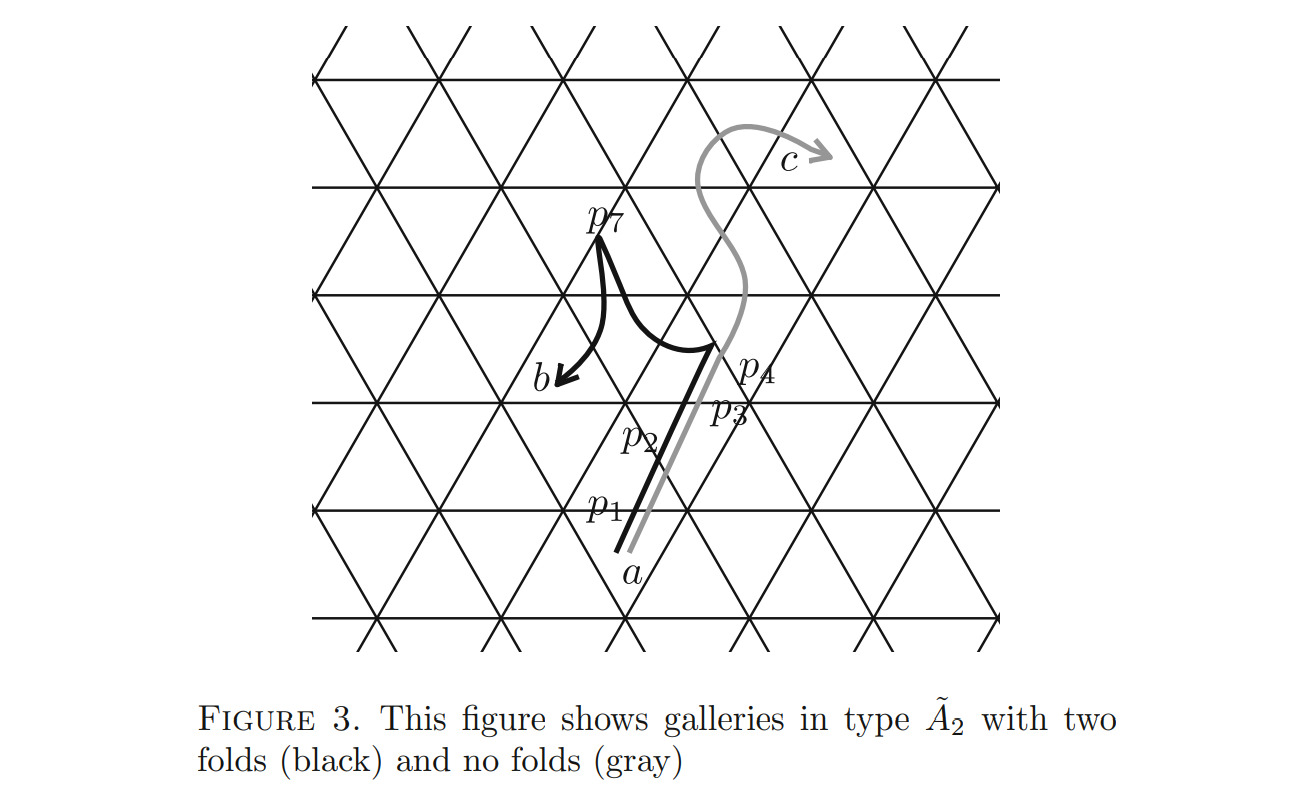
\includegraphics[scale=0.6]{Screenshot 2023-02-03 111653.png}\\

\begin{definition}
    Given a gallery $\gamma$ in \sg, and an orientation $\phi$, we say that $\gamma$ is \ix{positively folded} with respect to $\phi$ if, whenever $\gamma$ is folded at position $i$, $\phi(p_i,c_i)=+1$.  We can similarly define \ix{negatively folded}.
\end{definition}


\subsection{Galleries and Words}

\begin{definition}
    Consider a gallery $\gamma = (c_0,p_1,c_1,...,p_n,c_n)$. Let panel $p_i$ of $\gamma$ have type $s_{j_i}\in S$. We define its \ix{type} $\tau(\gamma)$ as the word 
    \[\tau(\gamma):=s_{j_1}...s_{j_n}.\]
    We denote by $\Gamma_{\phi}^+(w)$ the set of all $\phi$-positively folded galleries which have type $w$. 
\end{definition}

\begin{definition}
    The \ix{decorated type} $\hat\tau(\gamma)$ of a gallery $\gamma = (c_0,p_1,c_1,...,p_n,c_n)$ is the decorated word
    \[\hat\tau(\gamma):= s_{j_1}...\hat{s_{j_i}}...s_{j_n},\]
    where we place a hat on the elements $s_{j_i}$ of the word which correspond to a fold $c_{i-1}=c_i$ of the gallery. We denote by $\Gamma_{\phi}^+(\hat{w})$ the set of all $\phi$-positively folded galleries which have decorated type $\hat{w}$.
\end{definition}

\begin{lemma}
    Let $c_0$ be a fixed alcove in our Coxeter complex \sg. 
    \begin{enumerate}
        \item There is a bijection between words in $S$ and unfolded galleries starting at $c_0$.
        \item There is a bijection between decorated words in $S$ and gallleries starting at $c_0$. 
    \end{enumerate}
\end{lemma}

\begin{lemma}
    Let $\gamma$ be a gallery. Then
    \begin{enumerate}
        \item $F(\gamma)=\emptyset$ if and only if $\tau(\gamma)=\hat{\tau}(\gamma).$
        \item $\gamma$ is minimal if and only if $F(\gamma)=\emptyset$ and $\tau(\gamma)$ is reduced.
    \end{enumerate}
    \tr{What is the function F? I can't find the definition in this paper. Is it the set of all repeated chambers?}
\end{lemma}

We want to be able to characterise the last alcove in a gallery. We do this by constructing another gallary which removes any folds from our original gallery. This leads to an unfolded gallery which has shorter length than the original gallery.

\begin{definition}
    Consider a gallery $\gamma = (c_0,p_1,c_1,...,p_n,c_n)$ in \sg. We create a new gallery, called the \ix{footprint} \ix{ft}$(\gamma)$ \ix{of} $\gamma$, by deleting all pairs $p_i,c_i$ such that the letter $s_i$ has a hat in $\hat{\tau}(\gamma)$. 

\end{definition}

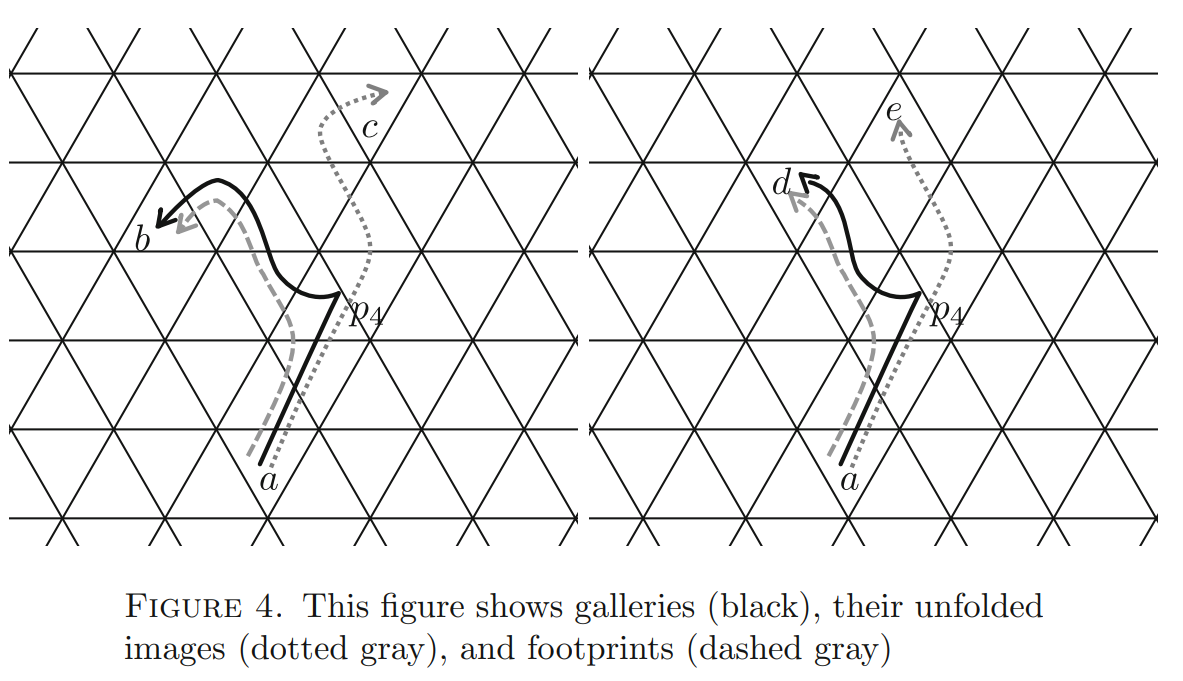
\includegraphics[scale=0.6]{Screenshot 2023-02-03 133522.png}\\

\begin{lemma}
    We can calculate the final alcove of a gallery as the element $c_n=c_0\cdot w$, where $w=\tau(\text{ft}(\gamma))$.
\end{lemma}

\subsection{Modification}

As $W$ has a natural left action on \sg, and so $W$ also acts on the set of galleries in \sg. For instance, $x\in W$ sends $\gamma = (c_0,p_1,c_1,...,p_n,c_n)$ to the gallery $\gamma = (xc_0,xp_1,xc_1,...,xp_n,xc_n)$. 

\begin{lemma}
    Consider an affine Coxeter system $(W,S)$ with a Coxeter complex \sg. Let $a$ be a chamber in the boundary complex $\partial\Sigma$. Now a gallery $\gamma$ is $\phi_a$-positively folded if and only if $x\cdot \gamma$ is $\phi_a$-positively folded. So the action of $W$ on $\partial\Sigma$ preserves the condition of '$\phi_a$-positively foldedness'.
\end{lemma}

\begin{definition}
    Consider a gallery $\gamma = (c_0,p_1,c_1,...,p_n,c_n)$. Let $H_i$ be the hyperplane containing the panel $p_i$, and let $r_i$ be the reflection across $H_i$. For $i=1,...,n$, let
    \[\gamma^i:=(c_o,p_1,...,p_i,r_ic_i,r_ip_{i+1},r_ic_{i+1},...,r_ip_n,r_ic_n).\]
    If $\gamma$ was folded at panel $p_i$, we call $\gamma^i$ a \ix{unfolding of }$\gamma$ at $p_i$. Otherwise, we call it a \ix{folding}.
\end{definition}

\begin{lemma}
    For all $i=1,...,n$, $\tau(\gamma)=\tau(\gamma^i)$. So folding and unfolding does not change the gallery type. Also, $(\gamma^i)^i=\gamma$. \tr{I can't quite see why reflections are type preserving?}
\end{lemma}

\begin{lemma}
    For all $i,j=1,...,n$, $(\gamma^i)^j=(\gamma^j)^i.$
\end{lemma}

Because of this property, we are able to define a \ix{multifolding} with respect to a subset $I$ of $\{1,...,n\}$ as the (un-)foldings $\gamma^I$. Now multifoldng does not affect the type. Then the set of folds of $\gamma^I$ will be the symmetric difference of the folds of $\gamma$ and $I$. In particular, if $I$ and $J$ are subsets of $\{1,...,n\}$, $(\gamma^I)^J=\gamma^{I\Delta J}$. 

\begin{corollary}
    Given any gallery $\gamma$, there is a subset $I\subset \{1,...,n\}$ such that $\gamma^I$ is unfolded, and $\gamma$ and $\gamma^I$ have the same type.
\end{corollary}


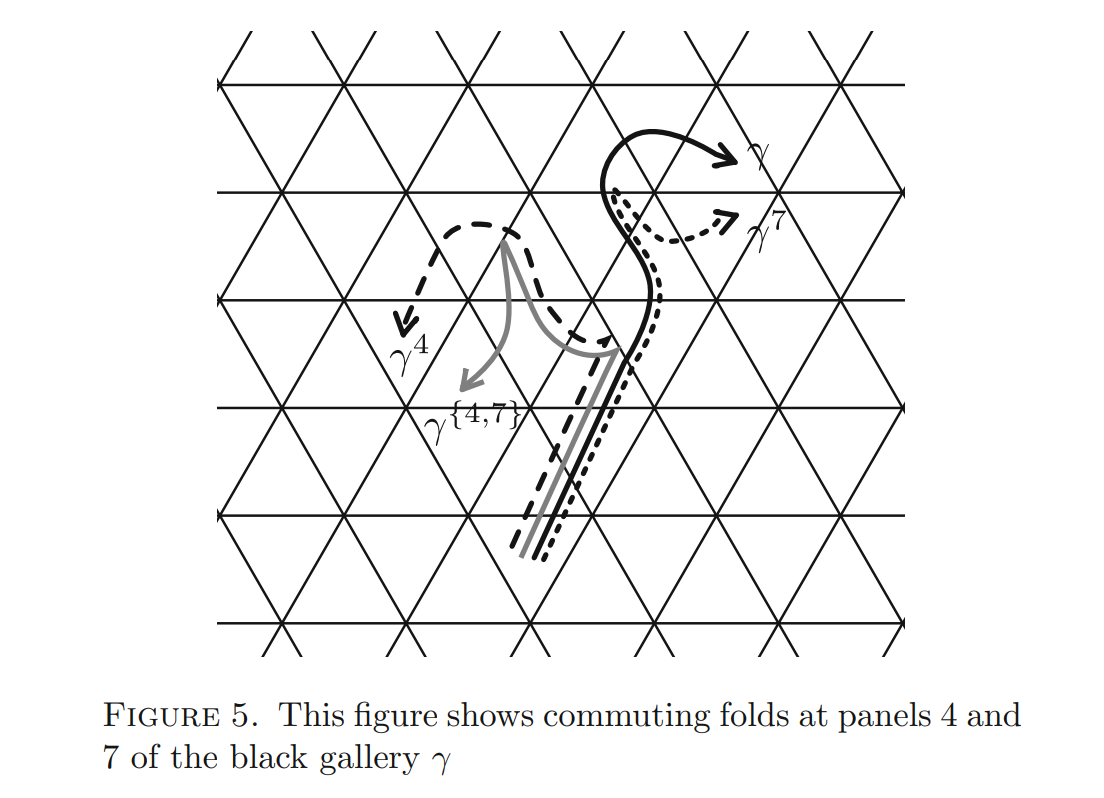
\includegraphics[scale=0.6]{Screenshot 2023-02-03 153412.png}\\


Now we fix an alcove of our Coxeter complex, and call this 1. Then, for any word $w$ with elements in $S$, we let $\gamma_w$ be the unique unfolded gallery which has type $w$ and starts at 1. Now we write
\begin{enumerate}
    \item $\gamma \rightharpoonup \eta$ if $\gamma$ and $\eta$ are galleries such that $\eta = \gamma^I$ for some index set $I$,
    \item $w\rightharpoonup u$ if $w$ and $u$ are words in $S$ such that there is a folding of $\gamma_w$ which has footprint $u$.
    \item $w\rightharpoonup x$ if $x$ is an element of $W$ such that there is a folding of $\gamma_w$ which has end alcove $c_x$. 
\end{enumerate}
We denote by $A\stackrel{\phi}{\rightharpoonup} B$ if the respective gallery is $\phi$-positively folded.

\subsection{Statistics on positive folds}

We now restrict to looking at Weyl chamber orientations over affine Coxeter complexes. This means that we have a complex \sg, with a boundary $\partial$\sg, and that our orientations are induced by a boundary chamber orientation. 

We want to calculate the number of positive folds we can make.

\begin{proposition}
    Consider the largest element $w_0$ in $W_0$. Given an $x\in W$, and a $\phi$-postive (multi)folding $\gamma$ of $\gamma_x$, we have
    \[l_R(xy^{-1})\leq |F(\gamma)|\leq l(w_0),\]
    where $y:=\tau($ft$(\gamma))$.
\end{proposition}
\tr{proof uses lemmas from [13], should I have a look at that resource?}

\begin{definition}
    Let $\mathcal{H}(\Sigma)$ be the set of all hyperplanes contained in our Coxeter complex. For an alcove $c$ of \sg, let $\mathcal{H}(c)$ be the subset of $\mathcal{H}(\Sigma)$ which separates $c$ and the fixed identity alcove 1. Now $\mathcal{H}(c)=\mathcal{H}_{\phi}^+(c)\sqcup \mathcal{H}_{\phi}^-(c)$. 
\end{definition}

\tr{When we refer to the 'Coxeter complex', are we including the space taken up by chambers, or is it just the panels in our tiling? For instance, in this definition, if the Coxeter complex spans the whole plane, techincally all the hyperplanes of the plane are in the complex? Or if the complex is finite there are technically no hyperplanes in the complex. }

\begin{definition}
    Let $Ch(\Sigma)$ denote the set of all alcoves in \sg. The $\phi$-valuation map is the map $\textnormal{v}_\phi:\textnormal{Ch}(\Sigma)\longrightarrow\mathbb{Z}$, with
    \[c\mapsto \textnormal{v}_\phi(c):= |\mathcal{H}_{\phi}^+(c)|-|\mathcal{H}_{\phi}^-(c)|.\]
\end{definition}

\begin{definition}
    Let $p_\phi : \textnormal{Ch}(\Sigma)\times \mathcal{H}\longrightarrow \{0,1\}$ be the function 
    \[p_\phi(c,H):= \begin{cases}
        1 & \textnormal{if $c$ is on a $\phi$-positive side of $H$,}\\
        0 & \textnormal{otherwise.}
    \end{cases}\]
\end{definition}

\begin{lemma}
    \[\textnormal{v}_\phi(c)=\sum_{H\in\mathcal{H}(\Sigma)}(p_{\phi}(c,H)-p_\phi(1,H)).\]
\end{lemma}

\begin{lemma}
    \[l(x)\geq\textnormal{v}_\phi(c_x).\]
\end{lemma}

\begin{definition}
    We call an alcove $c$ \ix{dominant} with respect to $\phi$ if $\textnormal{v}_\phi(c)=l(c).$
\end{definition}

\begin{lemma}
    \[l(x)=\max_{a\in W_0}\textnormal{v}_{\tilde{\phi}_a}(c_x).\]
\end{lemma}

\begin{lemma}
    Let $\phi\in$Dir$(W)$, $r\in W$ be a reflection across the hyperplane $H_r$ and $x\in W$. Then v$_\phi(x)>$v$_\phi(rx)$ if and only if $x$ lies in the $\phi$-positive side of $H_r$. 
\end{lemma}

\tr{Not sure about a step in the proof}





\section{Braid invariant orientations}

\begin{definition}
    Consider a Coxeter system $(W,S)$ and a corresponding Coxeter complex \sg. Let $\phi$ be an orientation on \sg. Then we say that $\phi$ is \ix{braid invariant} if, given any two braid equivalent words $w,w'$ in $S$ and any $x\in W$, $w\stackrel{\phi}{\rightharpoonup} x$ if and only if $w'\stackrel{\phi}{\rightharpoonup} x$. Then if $y\phi$ is braid invariant for all $y\in W$, $\phi$ is called \ix{strongly braid invariant}. 
\end{definition}


\begin{proposition}
    Weyl chamber orientations are braid invariant.
\end{proposition}

\section{Shadows}
\begin{definition}
    Consider a Coxeter system $W$ and an orientation $\phi$ on the Coxeter complex \sg\W. Let $w$ be a word is $S$. The \ix{shadow} of $w$ with respect to $\phi$ is the set 
    \[\textnormal{Sh}_\phi(w):=\{u\in W|w\stackrel{\phi}{\rightharpoonup} u\}.\]
    If $\phi$ is braid invariant, we can define Sh$_\phi(x)=$Sh$_\phi(w)$, where $w$ is any reduced expression of $x\in W$. If we have the Weyl chamber orientation $\phi_a$ with $a\in W_0$, the \ix{regular shadow} of $x$ with respect to $a$ is Sh$_a(w):=$Sh$_{\phi_a}(w)$. The \ix{full shadow} of $x$ is the union of regular shadows. 
\end{definition}

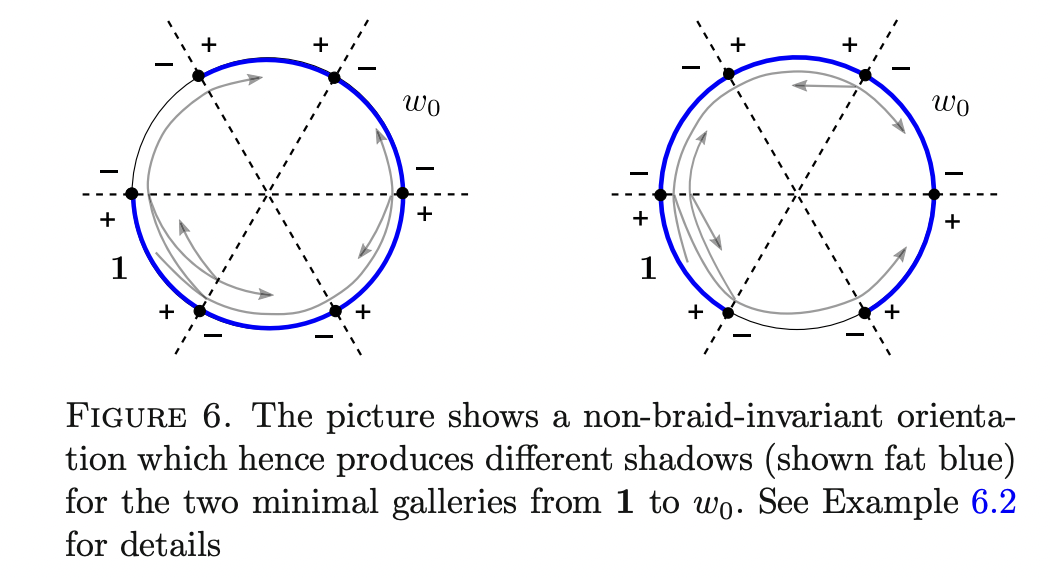
\includegraphics[scale=0.6]{Screenshot 2023-02-08 at 10.39.18.png}\\

\tr{Is there an efficient way to prove that we have correctly calculated the shadow? In these examples, we can just try all possibilities but I'm sure it gets much harder very quickly. Is there a way to prove that an alcove is never reached for instance?}

\begin{definition}
    Let $x=s_1...s_n$ be a reduced expression for $x\in W$. Let $y\in W$. We say that $y\leq x$ if there exists a reduced expression for $y$ of the form $s_{i_1}...s_{i_k}$ with $1\leq i_1\leq...\leq i_j\leq n$. This ordering is called the \ix{Bruhat order}.
\end{definition}

\begin{proposition}
    Consider the trivial positive orientation $\phi_+$, and the alcove orientation $\phi_1$ towards 1. For $x,y\in W$, $x\geq y$ if and only if $x\stackrel{\phi_+}{\rightharpoonup} y$, if and only if $x\stackrel{\phi_1}{\rightharpoonup} y$.
\end{proposition}


\section{Computation of regular shadows}

Let Dir$(W)$ represent the set of chambers in the bounday complex $\partial\Sigma$. We call elements of Dir$(W)$ \ix{directions in W}. 

\begin{theorem}
    Let $\phi\in$Dir$(W)$, $x\in W$ and $s\in S$. Then
    \begin{enumerate}
        \item If $s$ is in the right descent set $D_R(x)$ of $x$, then we have
        \[\textnormal{Sh}_\phi(x)=\textnormal{Sh}_\phi(xs)\cdot s \cup \{z\in \textnormal{Sh}_\phi(xs):\textnormal{v}_\phi(zs)<\textnormal{v}_\phi(z)\}.\]
        \item If $s$ is in the left descent set $D_R(x)$ of $x$, then we have
        \[\textnormal{Sh}_\phi(x)=\begin{cases}
            s\cdot \textnormal{Sh}_\phi(sx)\cup \textnormal{Sh}_\phi(sx) &if\textnormal{ v}_\phi(s)<0,\\
            s\cdot \textnormal{Sh}_\phi(sx) &if \textnormal{ v}_\phi(s)>0.\\
        \end{cases}\]
    \end{enumerate}
\end{theorem}

\tr{What is the left and right descent?}

\begin{definition}
    Given $x\in W$, $a\in W_0$ and $\phi\in$ Dir$(W)$, the \ix{partial shadow in local direction a} is the set 
    \[\textnormal{Sh}_\phi^a(x):=\{y\in \textnormal{Sh}_\phi(x)|\bar{y}=a\},\]
    where $\bar{y}$ is the image of $y$ under the natural projection to the spherical Weyl group $W_0$. 
\end{definition}


\begin{lemma}
    Let $\phi\in\textnormal{Dir}(W)$ and $x\in W$. Let $w=(s_1,...,s_n)$ be a reduced word for $x$. Let $A_0=\{1\}$ and let
    \[A_i:=A_{i-1}\cdot s_i\cup \{z\in A_{i-1}|v_\phi(zs)<v_\phi(z)\}.\]
    Then $A_n=\textnormal{Sh}_\phi(x)$. 
\end{lemma}

\begin{lemma}
    Let $\phi\in$ Dir$(W)$ and $x\in W$, with $(s_n,...,s_1)$ a reduced expression for $x$. Let $B_0^\phi:=\{1\}$ and define
    \[B_i^\phi = \begin{cases}
        s_iB_{i-1}^{s_i\phi}\cup B_{i-1}^\phi & \textnormal{if v}_\phi(s_i)<0,\\
        s_iB_{i-1}^{s_i\phi} & \textnormal{if v}_\phi(s_i)>0.
    \end{cases}\]
\end{lemma}



















































\end{document}